\documentclass[12pt]{article}

% Packages
\usepackage[utf8]{inputenc}
\usepackage{graphicx}
\usepackage{hyperref}
\usepackage[backend=biber,style=authoryear,citestyle=authoryear,natbib=true]{biblatex}
\addbibresource{references.bib}
\usepackage[a4paper, margin=0.8in]{geometry}
\usepackage{titlesec}
\setlength{\parskip}{1em} 
\setlength{\bibitemsep}{1em} % Add spacing between bibliography entries

%Customizing section titles
% Customize section and subsection titles
\titleformat{\section}
  {\normalfont\Large\bfseries} % Section titles will be in large, bold font
  {\thesection}{1em}{}
%   \titlespacing{\subsection}{0pt}{*0}{-0.8em}
  [\titlerule]
  

\titleformat{\subsection}
  {\normalfont\bfseries} % Subsection titles will be slightly smaller
  {\thesubsection}{1em}{}
\titlespacing{\subsection}{0pt}{0em}{-0.3em}

% Title
\title{Adaptation Plan Evaluation Report}
\author{Mukund Balaji Srinivas | u7274095}
\date{} % Remove the date 

\begin{document}

% Title Page
\maketitle

\begin{abstract}
This section provides a brief summary of the evaluation report, outlining the key question being addressed, methods used, and main conclusions.
\end{abstract}

\newpage

\section*{Introduction}
% \subsection*{Background}

The World Economic Forum (\cite{masterson_2024})  outlines six key technologies critical for climate change adaptation, 
including the powerful roles of Earth Observation [EO] and Artificial Intelligence [AI]. 


\subsection*{Context}
EO sector plays a pivotal role in climate change adaptation by offering critical data for monitoring deforestation, land-use changes, and rising sea levels (\cite{anderson_2017}). 
The EO technologies are essential for tracking progress towards the 2030 Agenda for Sustainable Development (\cite{unitednations_2015}), particularly in providing spatially explicit data to monitor targets across 
a wide range of SDGs [Sustainable Development Goals]. EO supports informed decision-making by governments and international 
organizations, allowing for better resource management and monitoring of the impact of climate mitigation strategies.
However, as EO becomes more industrialized (\cite{venkatesan_2020}) , it presents several significant environmental risks  
that must be considered when evaluating its contribution to climate adaptation (\cite{crisp_2020}). \\
While EO transitions to a more cloud-based data processing model, it introduces significant environmental 
considerations within the environmental science community. Storing and distributing EO data relies heavily on a global network of data centers, 
which are known to contribute substantially to carbon emissions and disproportionately use water resources. Despite these impacts, the specific 
environmental footprint of EO data centers remains opaque and requires critical assessment alongside its contributions to climate adaptation.(\cite{wilkinson_2024})

AI models require immense computational power and their energy demands continue to grow exponentially (\cite{amodei_2018}),
 their potential contribution to carbon emissions becomes a significant concern (\cite{taddeo_2021}). Nonetheless, leveraging AI’s 
 expanding capabilities to improve climate change mitigation is both feasible and crucial. 
 For instance, AI can be used to better understand the impacts of industrial production, construction, 
 and transportation on climate change, while also estimating the effectiveness of policy interventions such 
 as carbon taxes and carbon trading systems. However, ensuring the sustainable and equitable deployment of these 
 AI-driven solutions will require robust governance frameworks (\cite{taddeo_2021}).

 The  Information and Communication Technology [ICT] sector that encompasses EO and AI
is responsible for over 3 percent of the world's carbon emissions (\cite{jones_2018}) . Specifically , 
companies like Samsung and Amazon had a footprint of around 40,000MT of \(CO_2\) equivalent in 2021 (\cite{navarro_2023_the}) —raises the question 
of how big tech companies are addressing their environmental impact. While AI and EO tools offer potential benefits in 
mitigating climate change, their carbon costs are often overlooked.

% \newpage
Given the complexity of assessing the environmental impact of EO data collection (\cite{wilkinson_2024}) and storage coupled with the challenges in calculating AI's carbon 
footprint (\cite{Henderson_2020}) , accurately evaluating the broader environmental effects of the ICT sector is particularly difficult. In this context, we aim to systematically 
assess the environmental reports of major tech companies, including Meta, Apple, Amazon, Google, Nvidia, Samsung, as well as satellite companies like Planet Labs. 


assess the environmental reports of major tech companies, including Meta, Apple, Amazon, Google, Nvidia, Samsung, as well as satellite companies like Planet Labs.

\subsection*{Planned Adaptation}
The adaptation policies of tech companies in the ICT domain generally focus on two main strategies:
\begin{enumerate}
    \item \textbf{Improving Product Energy Efficiency} \\ Tech companies aim to design AI-powered products that are more energy-efficient. This includes optimizing the algorithms and 
    models themselves to reduce the computational power required. By improving the efficiency of AI models, these companies can lower the overall energy consumption during 
    the training and deployment stages of AI systems . For instance, companies like Google and Nvidia are working on creating more efficient hardware accelerators and AI 
    chips that perform computations using less power while delivering the same level of performance (\cite{google_2024_environmental} ; \cite{nvidia_2024}).
    \item \textbf{Improving Operational Energy Efficiency} \\ In addition to product improvements, companies are also focusing on making their operational processes more energy-efficient. This includes 
    transitioning to renewable energy sources for their data centers, improving cooling mechanisms, and reducing water use. many firms mentioned here have been investing in renewable energy 
    projects to power their AI research and data centers. (\cite{apple_2024_environmental};\cite{amazon_2023_amazon};\cite{meta_sustainability_2023};\cite{google_2024_environmental};\cite{nvidia_2024}) 
     
\end{enumerate}

%% Methods
\section*{Methods}

The adaptation policies of tech companies in ICT generally focus on two main strategies:
\begin{enumerate}
  \item \textbf{Improving Product Energy Efficiency} \\ This involves optimizing algorithms, models, and software to reduce the computational 
  power required for operations. Enhancing the efficiency of ICT systems lowers energy consumption 
  during key processes such as data analysis, training, and deployment stages, which are resource-intensive. AI systems are a significant part 
  of this, but other areas—such as large-scale data analytics, distributed computing, and cloud services—also contribute to energy use.

  
  
  \item \textbf{Operational Energy Efficiency} \\ This includes transitioning to renewable energy sources for their data centers, 
  improving cooling mechanisms, and reducing water use. Firms like Amazon and Meta have been investing in renewable energy projects 
  to power their AI research and data centers.
\end{enumerate}




\section*{Comparison}
Here, make the necessary comparisons based on the criteria from the Methods section. Discuss how different nations/regions/sectors perform according to these criteria. You may break this into subsections if there are multiple comparisons.

\section*{Discussion}
Synthesize the information you gathered from the comparisons. Discuss patterns, insights, and important findings based on the comparisons made.

\section*{Conclusion}
Summarize the main conclusions of your evaluation. Reflect on what the comparisons suggest about the criteria and any recommendations based on the results.

%%Appendix
\appendix
\section*{Figures}
\begin{figure}[h]
  \centering
  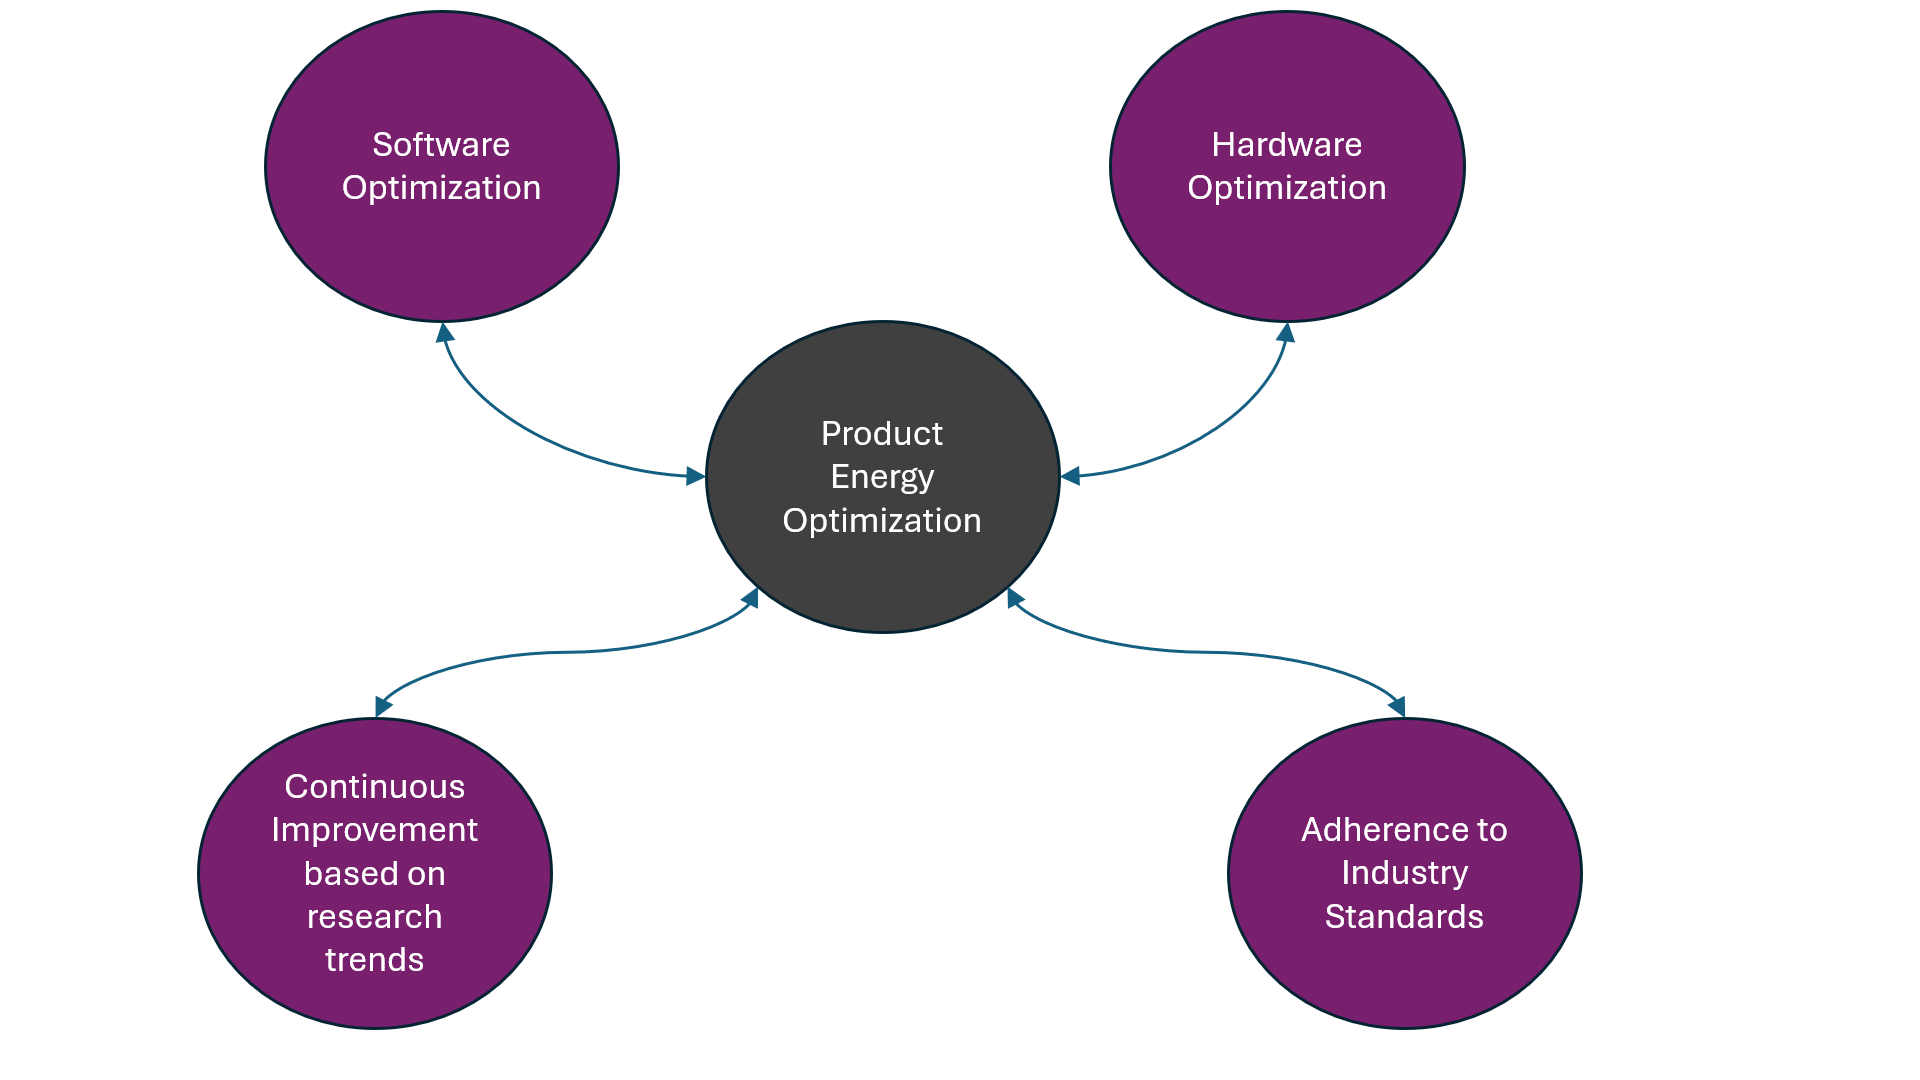
\includegraphics[width = \textwidth]{product_energy_optimization.png}
  \caption{Product Energy Optimization}
\end{figure}

\newpage
\printbibliography

\end{document}
